\documentclass[
  11pt,
  letterpaper,
   addpoints,
   answers
  ]{exam}

\usepackage{../exercise-preamble}
\usepackage{float}

\begin{document}

\noindent
\begin{minipage}{0.47\textwidth}

\includegraphics[width=\textwidth]{../fcfm_die}
\end{minipage}
\begin{minipage}{0.53\textwidth}
\begin{center}
\large\textbf{Análisis de Sistemas Dinámicos y Estimación} (EL3204-1) \\
\large\textbf{Clase auxiliar 2} \\
\normalsize Prof.~ Marcos Orchard - Sebastián Espinosa.\\
\normalsize Prof.~Aux.~Erik Sáez
\end{center}
\end{minipage}

\vspace{0.5cm}
\noindent
\vspace{.85cm}

\begin{questions}
    %%%%%%%%%%%%%%%%%%%%%%%%%%%
    \question Considere el siguiente circuito eléctrico, donde \(\alpha(t)i_2(t)\) corresponde al valor de la resistencia eléctrica de un potenciómetro, cuyo valor depende tanto de \(\alpha(t)\) como de la corriente que circula por el condensador, y \(v_{out}(t)\) (voltaje en el condensador) se mide con un voltímetro.
\begin{figure}[ht]
        \centering
        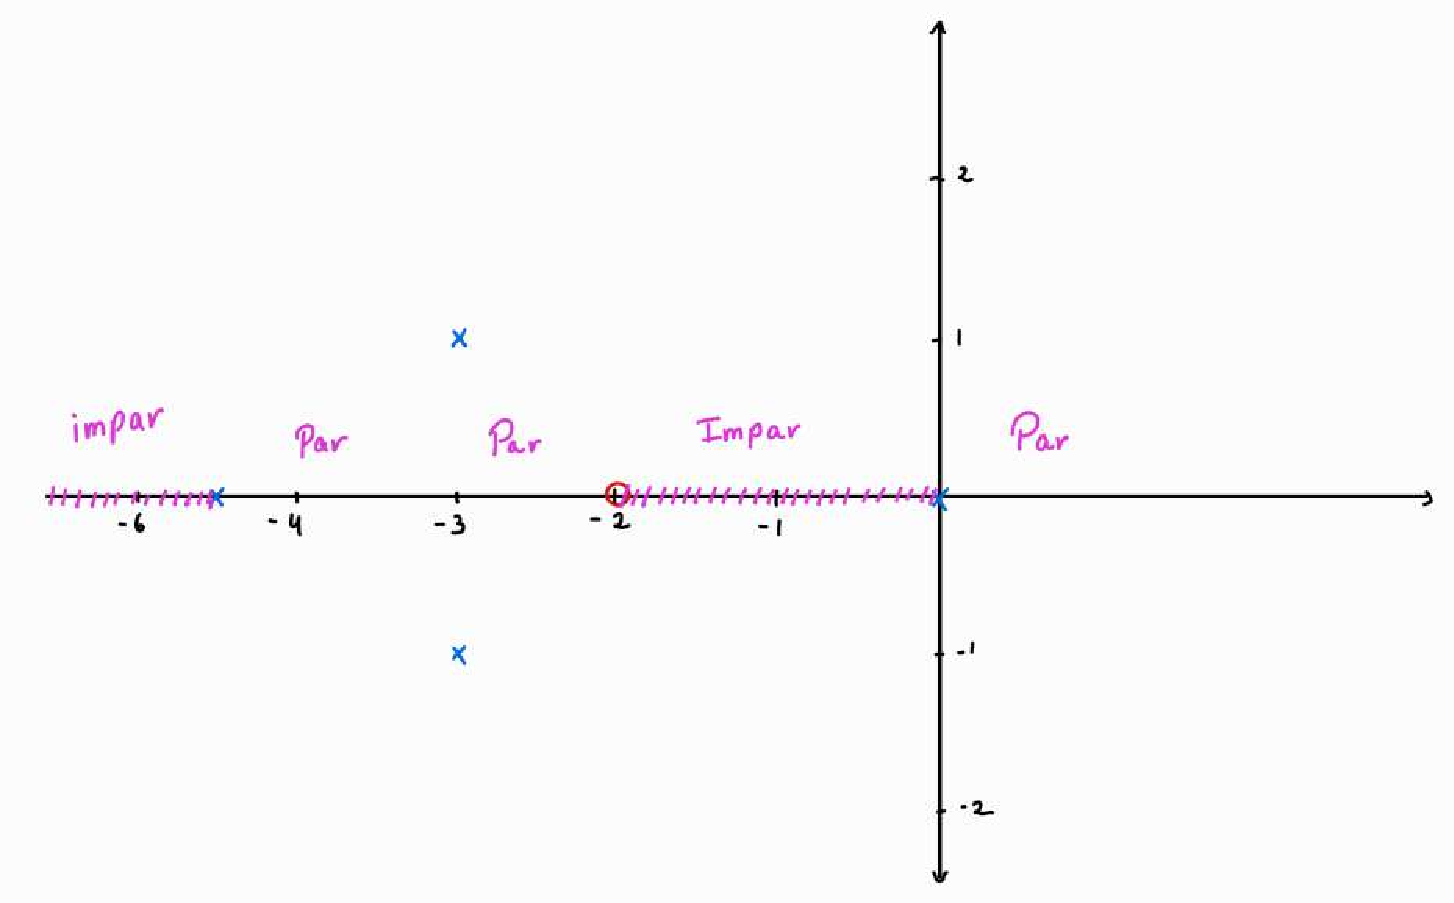
\includegraphics[width=0.6\textwidth]{Auxiliar_2_1}
    \end{figure}
\begin{enumerate}
    \item Establezca claramente el listado de hipótesis simplificatorias que permitan
    establecer un modelo matemático válido para este sistema. Indique las condiciones de borde y/o
    iniciales necesarias.
    \item Formule un modelo para el sistema en ecuaciones de estado.
    \item Caracterice completamente el modelo utilizando todos los puntos de vista descritos en clases.
    Clasifique todas las variables del sistema.
    \item Encuentre estado(s) cero, estado(s) de equilibrio y el estado tierra (de existir).
    \item Linealice el sistema en torno al (los) estado(s) de equilibrio encontrados.
\end{enumerate}
    %%%%%%%%%%%%%%%%%%%%%%%%%%%
\begin{solution}
\subsection*{Resolución 1.1}
Para poder formular un modelo del sistema, debemos primeramente considerar hipótesis simplificatorias que permitan simplificar el problema o establecer límites sobre las distintas restricciones del mismo; por lo tanto:
\begin{itemize}
    \item Los parámetros \(V_{in},\,R,\,R_0,\,C\) son constantes del sistema.
    \item El circuito opera en régimen de \emph{parámetros concentrados}.
    \item Se desprecia la resistencia interna del voltímetro.
    \item No se consideran efectos parásitos ni ruidos.
    \item \dots
\end{itemize}
Por otra parte, por conocimiento de circuitos se sabe que la condición inicial necesaria para determinar el estado del sistema corresponde al voltaje inicial del condensador \(v_c(0)\).
\subsection*{Resolución 1.2}
Primero se aplica la Ley de Corrientes de Kirchhoff (LCK) en el nodo superior, con lo que se tiene \(I(t)=i_1(t)+i_2(t)\). Además, utilizando la Ley de Voltajes de Kirchhoff (LVK) en la malla izquierda, se obtiene:
\begin{align}
V_{in}=RI+v_c \;=\; R i_1 + R i_2 + v_c .
\end{align}
Recordando la ecuación del condensador, \(i_C=C\,\dot v_c\), e identificando \(i_C=i_2\),
\begin{align}
V_{in}=R i_1 + RC\,\dot v_c + v_c .
\end{align}
En la rama de la derecha luego se tiene:
\begin{align}
v_c = R_0 i_1 + (\alpha\, i_2) i_1
    = R_0 i_1 + \alpha C \dot v_c\, i_1
    = \bigl(R_0 + \alpha C \dot v_c \bigr) i_1,
\end{align}
Despejando,
\begin{align}
i_1=\frac{v_c}{R_0+\alpha C \dot v_c}.
\end{align}
Sustituyendo la ecuación~(4) en la ecuación~(2) con el propósito de expresar todo en función de una única variable \(v_{c}\), se llega a:
\begin{align}
V_{in}= \frac{R\,v_c}{R_0+\alpha C \dot v_c} + RC\,\dot v_c + v_c .
\end{align}
Reordenando y desarrollando,
\begin{align}
R_0 V_{in}+ \alpha C V_{in}\dot v_c
= Rv_c + R_0 RC \dot v_c + \alpha RC^2 \dot v_c^{\,2} + R_0 v_c + \alpha C v_c \dot v_c ,
\end{align}
lo que lleva a la ecuación cuadrática en \(\dot v_c\):
\begin{align}
\alpha RC^2 \dot v_c^{\,2} + \bigl(R_0RC + \alpha C (v_c - V_{in})\bigr)\dot v_c
+ (R+R_0) v_c - R_0 V_{in} = 0.
\end{align}
Resolviendo para \(\dot v_c\),
\begin{align}
\dot v_c
= \frac{-\bigl(R_0RC + \alpha C (v_c - V_{in})\bigr) \pm \sqrt{S}}
       {2\alpha RC^2},
\end{align}
donde, por conveniencia,
\begin{align}
S
&= R_0^2 R^2 C^2
+ 2\alpha R_0 R C^2 (v_c - V_{in})
+ \alpha^2 C^2 (v_c - V_{in})^2 \nonumber\\
&\quad - 4\alpha R C^2 (R+R_0) v_c
+ 4 R_0 R C^2 V_{in}.
\end{align}
Alternativamente, dividiendo por \(RC\),
\begin{align}
\dot v_c
&= \frac{V_{in}-v_c}{2RC} - \frac{R_0}{2\alpha C} \nonumber\\
&\quad \pm \frac{1}{2\alpha C}\sqrt{
  R_0^2 + \frac{2\alpha R_0}{R}(v_c - V_{in})
  + \frac{\alpha^2}{R^2}(v_c - V_{in})^2
  - \frac{4\alpha (R+R_0)}{R} v_c + \frac{4R_0}{R}V_{in} } .
\end{align}
Con lo que se obtiene finalmente la ecuación diferencial que caracteriza el sistema, la cual es evidentemente \textbf{no lineal}.
\subsection*{Resolución 1.3}
Existen diversas características con las que podemos clasificar los modelos, algunas de estas son las siguientes:
\begin{center}
\begin{tabular}{|p{3cm}|p{11cm}|}
\hline
\textbf{Característica} & \textbf{Clasificación} \\
\hline
Origen & Fenómeno \emph{artificial} (sistema eléctrico construido). El sistema corresponde a un fenómeno \emph{artificial} porque es un sistema eléctrico diseñado y construido por el ser humano para un propósito específico. Los sistemas eléctricos no se encuentran en la naturaleza. \\
\hline
Naturaleza & \emph{Determinístico} (no se consideran ruidos \(w(t)\) o \(v(t)\)). El sistema es \emph{determinístico} porque no involucra variables aleatorias como ruido de proceso o de medición. Esto implica que el comportamiento del sistema está completamente determinado por sus entradas y condiciones iniciales. No hay incertidumbre en el sistema. \\
\hline
Número de variables & \emph{Monovariable} (un estado). El sistema depende de una sola variable de estado, que es el voltaje \(v_C\) en el condensador. El sistema no tiene múltiples estados que lo definan, lo que simplifica su análisis y control. \\
\hline
Continuidad & \emph{Continuo} (aparece \(\dot v_c\)). El sistema es \emph{continuo} porque la ecuación de estado involucra derivadas respecto al tiempo, lo que significa que sus variables cambian de manera continua en el tiempo. Esto implica que el sistema se modela con ecuaciones diferenciales. \\
\hline
Comportamiento espacial & \emph{Parámetros concentrados}. El sistema no depende de la localización espacial de los componentes dentro del sistema. Todos los parámetros (como la resistencia y el voltaje) se consideran concentrados en los componentes del circuito, sin tener en cuenta las posibles distribuciones espaciales. \\
\hline
Comportamiento temporal & \emph{Invariante en el tiempo}. El sistema no depende del momento en que se inicie el proceso, sino únicamente de las condiciones iniciales y las entradas. No hay efectos que cambien con el tiempo de inicio del sistema, lo que hace que el comportamiento sea predecible independientemente del instante de inicio. \\
\hline
Linealidad & \emph{No lineal} (por la dependencia racional en \(\dot v_c\)). El sistema es \emph{no lineal} debido a la dependencia racional en la ecuación de estado. La relación entre las entradas y las salidas no es directamente proporcional, lo que se debe a la presencia de términos no lineales en las ecuaciones que describen el sistema. \\
\hline
Realizabilidad & \emph{Causal y realizable}. El sistema es \emph{causal}, ya que la salida en cualquier instante solo depende de las condiciones pasadas y actuales, no de las futuras. Esto implica que el sistema puede implementarse físicamente, ya que no depende de información futura para determinar su comportamiento. \\
\hline
\end{tabular}
\end{center}



Además, deberemos definir las variables del sistema, las cuales se pueden definir de la siguiente manera:
\begin{itemize}
    \item Estado: \(x(t)=v_c(t)\).
    \item Salida: \(y(t)=v_{out}(t)=v_c(t)=x(t)\).
    \item Entrada: \(u(t)=\alpha(t)\).
\end{itemize}
Es importante recordar que la elección de la salida es, por lo general, arbitraria a menos que se indique específicamente en el enunciado.
\subsection*{Resolución 1.4}
A continuación se analizan los diferentes estados del sistema:

\begin{itemize}
  \item \textbf{Estado cero.} Un estado cero \(x_0 \in \Sigma\) es aquel tal que, $\forall$ \(t_0\), la salida instantánea bajo entrada nula satisface
  \begin{equation*}
    \forall\, t_0:\; y(t_0) \,=\, \overline{A}(x_0,0) \,=\, 0.
  \end{equation*}
  Esta definición es \emph{atemporal}: se refiere a una propiedad puntual de la relación estado–salida y no a la evolución posterior en el tiempo.
  En este sistema en particular, como \(y=v_C=x\), el estado cero es \(x_0 = 0\).

    \item \textbf{Estado de equilibrio.} Recordemos que un estado de equilibrio \(x_e \in \Sigma\) es tal que \(x_e = \overline{B}(x_e, 0)\). Esto significa que bajo entrada cero lo que implica que \(\alpha x=0\), si el sistema está en estado de equilibrio, entonces permanecerá en este estado por siempre. Para encontrarlo, buscamos \(x_e\) tal que \(\dot x=0\). Evaluando esta condición en la ecuación cuadrática se obtiene:
    \begin{center}
        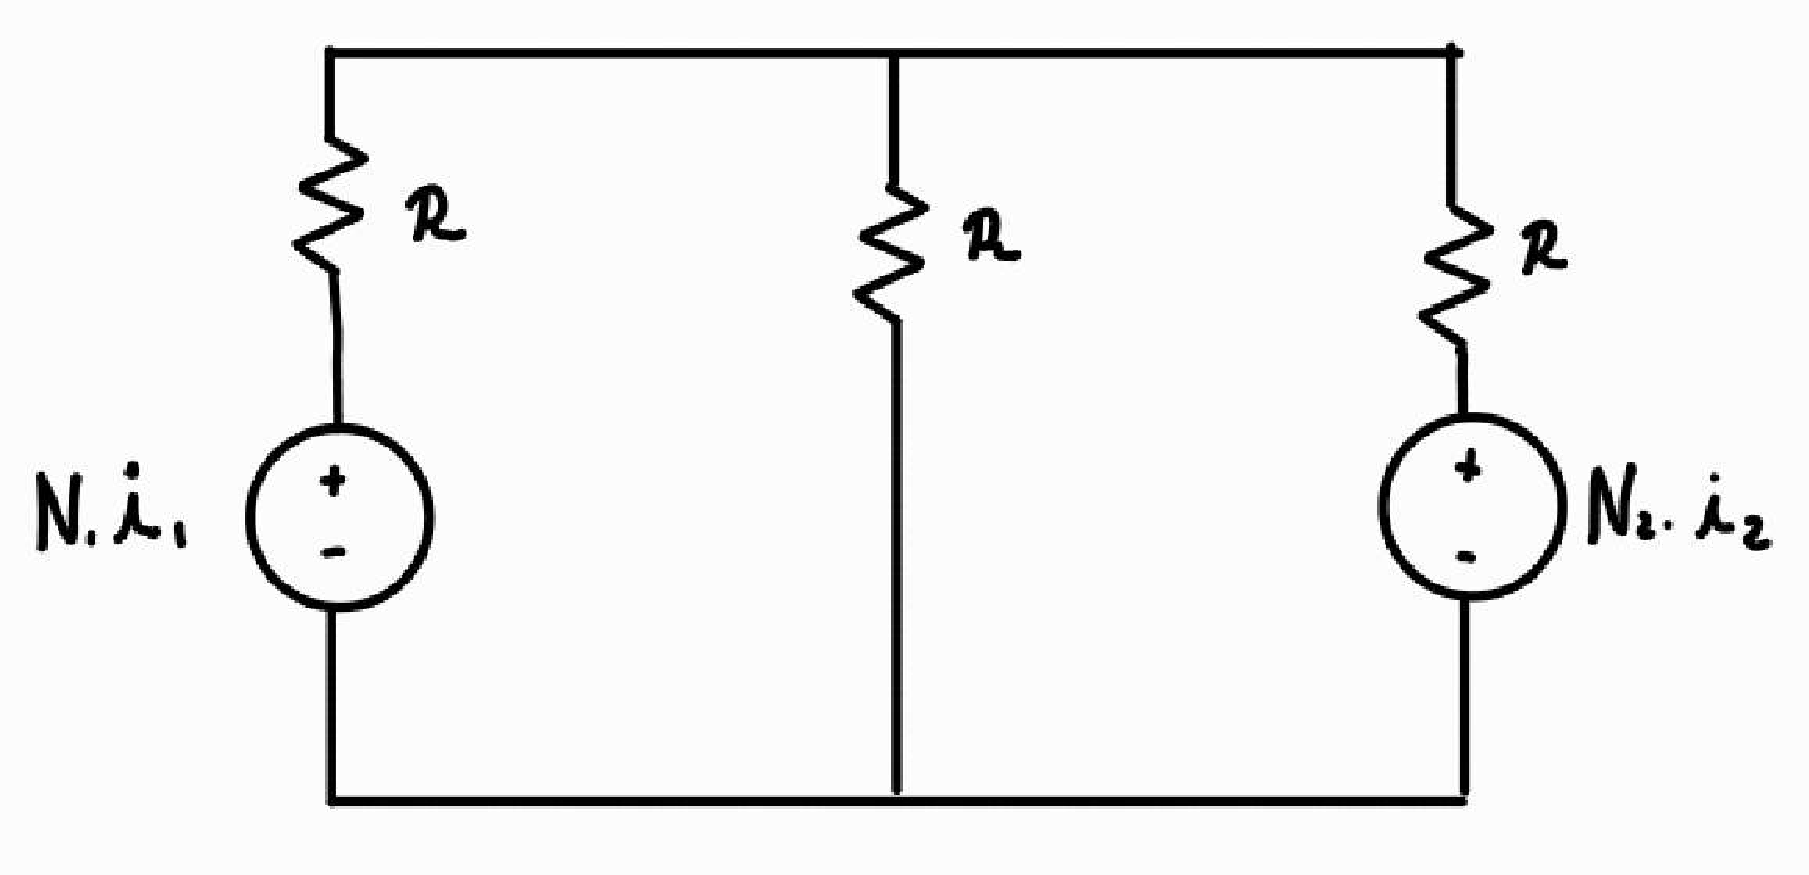
\includegraphics[width=0.6\textwidth]{Auxiliar_2_2}
    \end{center}
    Con lo que analizando la malla tenemos:
    \begin{align}
        V_{in} &= IR + R_{0}i_{1}\\
                &= i_{1}R + i_{2}R + R_{0}i_{1}\\
                &= (R + R_0)i_{1} + i_{2}R.\\
                &=(R + R_0)i_{1} + RC\dot{v_{c}}.\\
                &= (R + R_0)i_{1}\\
    \end{align}
    Anteriormente teníamos que $i_{1} = \frac{v_{c}}{R_{0}+\alpha C \dot{v_{c}}}$ y dado que $\alpha=\dot{v}_{c}=0$, por otro lado tendremos que el estado de equilibrio será $x_e = v_c$, podemos escribir
    \begin{align}
    (R+R_0)\,x_e - R_0 V_{in}=0 \quad \Rightarrow \quad
    x_e = \frac{R_0}{R+R_0}\,V_{in}.
    \end{align}
    
    \item \textbf{Estado tierra.} Recordemos que un estado tierra \(x_t \in \Sigma\) de un sistema es tal que \(\forall x_0 \in \Sigma, \lim_{t \to \infty} \overline{B}(x_0, 0) = x_t\). El estado tierra es aquel al cual converge el sistema para toda condición inicial y con entrada cero. Cuando el condensador está completamente cargado (en tiempo suficientemente grande), no conduce corriente y el circuito equivale a un divisor de tensión. Por lo tanto,
    \begin{align}
    x_t = \frac{R_0}{R+R_0}\,V_{in}.
    \end{align}
\end{itemize}

\subsection*{Resolución 1.5}
Buscamos linealizar el sistema, esto con el motivo de obtener un modelo más simple que capture la dinámica del sistema cerca de algún punto de operación que definamos nosotros previamente. 

\begin{align}
\dot{\tilde{x}} &= 
\left.\frac{\partial f}{\partial x}\right|_{\bar{x},\bar{u}} \tilde{x} 
+ \left.\frac{\partial f}{\partial u}\right|_{\bar{x},\bar{u}} \tilde{u}, \\[6pt]
\tilde{y} &= 
\left.\frac{\partial g}{\partial x}\right|_{\bar{x},\bar{u}} \tilde{x} 
+ \left.\frac{\partial g}{\partial u}\right|_{\bar{x},\bar{u}} \tilde{u}.
\end{align}
Donde tenemos que diferenciar correctamente que:
\begin{align}
    x &\coloneqq \text{Estado}\\
    \bar{x} &\coloneqq \text{Estado de operación}\\
    \tilde{x} &\coloneqq \text{Perturbación}
\end{align} 
Lo mismo aplica para u, luego podemos definir la relación entrada-salida del sistema como $f(x,u) = f(v_{c},\alpha)$ y $g(x,u) = g(v_{c},\alpha)$. Luego tenemos que estas corresponden a lo siguiente:
{\small
\begin{align}
f(v_C,\alpha)
&= \frac{V_{in}-v_C}{2RC}
   - \frac{R_0}{2\alpha C}
   - \frac{1}{2\alpha C}\,\sqrt{%
        R_0^2
        + 2\alpha\,\frac{R_0}{R}\,(v_C - V_{in})
        + \frac{\alpha^2}{R}\,(v_C - V_{in})^2
        - \frac{4\alpha (R+R_0)}{R}\,v_C
        + \frac{4R_0 V_{in}}{R}
     }, \\[6pt]
g(v_C,\alpha) &= v_C.
\end{align}
}


Consideramos el valor negativo de la raíz en la expresión anterior (elección arbitraria). Luego tenemos que calcular las derivadas vistas anteriormente, por lo tanto:
\begin{align}
\frac{\partial f}{\partial v_C} 
&= -\frac{1}{2RC} 
   - \frac{1}{4 \alpha C \sqrt{S}}
      \left[ 
        2 \alpha \frac{R_0}{R} 
        + 2 \alpha^2 (v_C - V_{in}) 
        - \frac{4 \alpha (R+R_0)}{R} 
      \right] \\[6pt]
&= -\frac{1}{2RC} 
   - \frac{1}{2RC \sqrt{S}}
      \left[ 
        R_0 + \frac{\alpha}{R}(v_C - V_{in}) - 2(R+R_0) 
      \right]
\end{align}
Donde tenemos que $S$ equivale a:

\begin{equation}
S = R_0^2 + 2\alpha \frac{R_0}{R} (v_C - V_{in}) + \alpha^2 \frac{(v_C - V_{in})^2}{R} - 4\alpha \frac{(R + R_0)}{R} v_C + \frac{4R_0 V_{in}}{R}
\end{equation}

Por otra parte, calculando la derivada con respecto a \(\alpha\) tenemos

\begin{align}
\frac{\partial f}{\partial \alpha} 
&= \frac{R_0}{2\alpha^2 C} 
   - \frac{1}{2C} \frac{\partial}{\partial \alpha} 
     \sqrt{R_0^2 
     + 2R_0 \frac{1}{\alpha^2 R} (v_C - V_{in}) 
     + (v_C - V_{in})^2 \frac{R_0}{R^2} 
     - 4(R + R_0) v_C \frac{1}{\alpha R} 
     + \frac{4R_0 V_{in}}{\alpha^2 R}} \\[6pt]
&= \frac{R_0}{2\alpha^2 C} 
   - \frac{1}{4C \sqrt{K}} 
     \left[
       - \frac{2R_0^2}{\alpha^3}
       - \frac{2R_0}{\alpha^2}(v_C - V_{in})
       + \frac{4(R + R_0)v_C}{\alpha^2 R}
       - \frac{8R_0 V_{in}}{\alpha^3 R}
     \right]
\end{align}


donde tenemos que K corresponde a:

\begin{equation}
K = \frac{R_0^2}{\alpha^2} + 2 \frac{R_0}{\alpha^2 R} (v_C - V_{in}) + \frac{(v_C - V_{in})^2}{R^2} - 4 \frac{(R + R_0)}{R} v_C + \frac{4R_0 V_{in}}{R}
\end{equation}

Para simplificar, en la ecuación (31) saquemos el término \(\alpha^2\) del denominador, de modo que si definimos \(K'\) como:

\begin{equation}
K' = R_0^2 + 2R_0 \frac{\alpha}{R} (v_C - V_{in}) + \frac{\alpha^2 (v_C - V_{in})^2}{R^2} - 4\alpha (R + R_0) v_C \frac{1}{R} + \frac{4R_0 V_{in}}{R}
\end{equation}

Entonces podemos ver que \(K' = S\), por lo que

\begin{align}
\frac{\partial f}{\partial \alpha} 
&= \frac{R_0}{2\alpha^2 C} 
   - \frac{1}{4 C \sqrt{K}}
     \left[
       \frac{2R_0^2}{\alpha^3}
       - \frac{2R_0}{\alpha^2 R}(v_C - V_{in})
       + \frac{4(R+R_0)v_C}{\alpha^2 R}
       - \frac{8R_0 V_{in}}{\alpha^3 R}
     \right] \\[6pt]
&= \frac{R_0}{2\alpha^2 C} 
   - \frac{\alpha}{4 C \sqrt{S}}
     \left[
       \frac{2R_0^2}{\alpha^3}
       - \frac{2R_0}{\alpha^2 R}(v_C - V_{in})
       + \frac{4(R+R_0)v_C}{\alpha^2 R}
       - \frac{8R_0 V_{in}}{\alpha^3 R}
     \right] \\[6pt]
&= \frac{R_0}{2\alpha^2 C} 
   - \frac{1}{4 C \sqrt{S}}
     \left[
       \frac{2R_0^2}{\alpha^2}
       - \frac{2R_0}{\alpha R}(v_C - V_{in})
       + \frac{4(R+R_0)v_C}{\alpha R}
       - \frac{8R_0 V_{in}}{\alpha^2 R}
     \right] \\[6pt]
&= \frac{1}{2\alpha^2 C}
   \left\{
     R_0 - \frac{1}{2\sqrt{S}}
     \left[
       -2R_0^2
       - \frac{2\alpha R_0}{R}(v_C - V_{in})
       + \frac{4\alpha(R+R_0)v_C}{R}
       - \frac{8R_0 V_{in}}{R}
     \right]
   \right\}
\end{align}

Luego, las derivadas sobre \(g(v_C, \alpha)\) son directas, es decir,

\begin{equation}
\frac{\partial g}{\partial v_C} = 1, \quad \frac{\partial g}{\partial \alpha} = 0
\end{equation}

Finalmente, para obtener el sistema linealizado debemos evaluar estas derivadas en el punto de operación. Como punto de operación consideraremos \(\bar{v} = \frac{R_0}{R + R_0} V_{in}\), y para evitar divergencias, consideraremos \(\bar{\alpha} = 1\). Evaluando cada derivada, tenemos

\begin{equation}
A = \left. \frac{\partial f}{\partial v_C} \right|_{\bar{v_C}, \bar{\alpha}}
\end{equation}

Para evaluar \(A\), consideremos que si evaluamos \(S\) en el punto de operación, tenemos
\begin{align}
S &= R_0^2 
   + 2\alpha \frac{R_0}{R}(v_C - V_{in})
   + \frac{\alpha^2}{R}(v_C - V_{in})^2
   - \frac{4\alpha (R+R_0)}{R} v_C
   + \frac{4R_0 V_{in}}{R} \\[6pt]
&= R_0^2 
   + 2 \frac{R_0}{R}\left(\frac{R}{R+R_0}-1\right)V_{in}
   + \frac{1}{R}\left(-\frac{R}{R+R_0}V_{in}\right)^2
   - \frac{4(R+R_0)}{R}\frac{R_0}{R+R_0}V_{in}
   + \frac{4R_0 V_{in}}{R} \\[6pt]
&= R_0^2 
   - 2 \frac{R_0}{R+R_0}V_{in}
   + \left(\frac{V_{in}}{R+R_0}\right)^2 \\[6pt]
&= \left( R_0 - \frac{V_{in}}{R+R_0} \right)^2
\end{align}


Luego, usando este valor para calcular \(A\), tenemos

\begin{align}
A &= -\frac{1}{2RC} 
     - \frac{1}{2RC\sqrt{S}}
       \left[ 
         R_0 + \frac{\alpha}{R}(v_C - V_{in}) - 2(R+R_0) 
       \right] \bigg|_{v_C,\alpha} \\
&= -\frac{1}{2RC} 
   - \frac{1}{2RC \left( R_0 - \tfrac{V_{in}}{R+R_0} \right)}
     \left[
       R_0 - \frac{V_{in}}{R+R_0} - 2R - 2R_0
     \right] \\
&= -\frac{1}{2RC} 
   + \frac{1}{2RC \left( R_0 - \tfrac{V_{in}}{R+R_0} \right)}
     \left[
       R_0 + 2R + \frac{V_{in}}{R+R_0}
     \right]
\end{align}

Por otra parte, al calcular \(B\) tenemos

\begin{align}
B &= \left. \frac{\partial f}{\partial \alpha} \right|_{v_C, \alpha} \\[6pt]
&= \frac{1}{2\alpha^2 C} \left\{ 
     R_0 - \frac{1}{\sqrt{S}}
     \left[
       -R_0^2 - \frac{\alpha R_0}{R}(v_C - V_{in})
       + \frac{2\alpha(R+R_0)}{R}v_C 
       - \frac{4R_0 V_{in}}{R}
     \right]
   \right\}\bigg|_{v_C,\alpha} \\[6pt]
&= \frac{1}{2C} \left\{
     R_0 - \frac{1}{R_0 - \tfrac{V_{in}}{R+R_0}}
     \left[
       -\frac{R_0^2}{R} - \frac{R_0}{R}\!\left(-\frac{R}{R+R_0}V_{in}\right)
       + \frac{2(R+R_0)}{R}\frac{R_0}{R+R_0}V_{in}
       - \frac{4R_0 V_{in}}{R}
     \right]
   \right\} \\[6pt]
&= \frac{1}{2R_0 C} 
   - \frac{1}{2C\!\left(R_0 - \tfrac{V_{in}}{R+R_0}\right)}
     \left[
       -R_0^2 + \frac{R_0}{R+R_0}V_{in}
       + \frac{2R_0}{R}V_{in}
       - \frac{4R_0}{R}V_{in}
     \right] \\[6pt]
&= \frac{1}{2R_0 C} 
   - \frac{1}{2C\!\left(R_0 - \tfrac{V_{in}}{R+R_0}\right)}
     \left[
       \frac{R_0}{R+R_0}V_{in} - 2\frac{R_0}{R}V_{in} - R_0^2
     \right]
\end{align}

Finalmente, utilizando estos valores podemos definir el sistema linealizado como

\begin{align}
\dot{\tilde{x}} &= A\tilde{x} + Bu\\
\tilde{y} &= \tilde{x} 
\end{align}

\end{solution}


    %%%%%%%%%%%%%%%%%%%%%%%%%%%
    \question Considere el sistema linealizado del auxiliar anterior, modelado por la siguiente ecuación diferencial:
    \begin{equation}
        \ddot{\theta}(t) = \frac{g}{l} \theta(t) + \frac{1}{l} u(t)
    \end{equation}

    \begin{enumerate}
        \item Descomponer la salida como la suma de la respuesta a condiciones iniciales nulas y la respuesta a entrada nula en el dominio de Laplace.
        \item Obtener la función de transferencia del sistema y encontrar la respuesta al impulso con condiciones iniciales nulas en el dominio del tiempo.
        \item Obtener la respuesta a entrada nula en el dominio del tiempo, y expresar la respuesta para una entrada y condiciones iniciales arbitrarias.
        \item Encuentre la salida cuando la entrada es un escalón unitario
    \end{enumerate}

%%%%%%%%%%%%%%%%%%%%%%%%%%%
\begin{solution}
\subsection*{Resolución 2.1}
Para realizar la descomposición, trabajemos en el dominio de Laplace debido a que dicho dominio facilita el análisis de sistemas lineales. Aplicando la transformada de Laplace sobre la ecuación diferencial del sistema, se tiene:
\begin{equation}
\mathcal{L}\left\{ \ddot{\theta} \right\} = s^2\Theta(s) - s\theta(0) - \dot{\theta}(0),
\end{equation}
donde los términos $\theta(0)$ y $\dot{\theta}(0)$ representan las condiciones iniciales del sistema. A continuación:
\begin{equation}
s^2\Theta(s) - s\theta(0) - \dot{\theta}(0) = \frac{g}{l} \Theta(s) + \frac{1}{l} U(s).
\end{equation}

Reordenando para despejar el término de la salida, tenemos:

\begin{equation}
\Theta(s) = \frac{s\theta(0) + \dot{\theta}(0)}{s^2 - \frac{g}{l}} + \frac{1}{l} \frac{1}{s^2 - \frac{g}{l}} U(s),
\end{equation}

donde podemos ver que la salida \(\Theta(s)\) está escrita como la suma de dos términos. El primero de ellos corresponde a:

\begin{equation}
\Theta_0(s) = \frac{s\theta(0) + \dot{\theta}(0)}{s^2 - \frac{g}{l}},
\end{equation}

y corresponde a la salida cuando se tienen condiciones iniciales arbitrarias pero entrada nula, denominada RENC (Respuesta a Entrada Nula o Cero). El segundo término es:

\begin{equation}
\Theta_s(s) = \frac{1}{l} \frac{1}{s^2 - \frac{g}{l}} U(s),
\end{equation}

y corresponde a la salida cuando utilizamos condiciones iniciales nulas pero una entrada arbitraria, denominada RESC (Respuesta a Estado Cero). Así, podemos ver que:
\begin{equation}
\Theta(s) = \Theta_0(s) + \Theta_s(s),
\end{equation}

\subsection*{Resolución 2.2}
La noción de función de transferencia está estrechamente ligada con la RESC, ya que para obtener la función de transferencia, asumimos condiciones iniciales nulas y una entrada arbitraria. Bajo estos supuestos, tenemos:

\begin{equation}
\Theta(s) = \frac{1}{l} \frac{1}{s^2 - \frac{g}{l}} U(s).
\end{equation}

A continuación, la función de transferencia \(H(s)\) del sistema se define como:

\begin{equation}
H(s) = \frac{\Theta_s(s)}{U(s)},
\end{equation}
donde es importante notar que utilizamos la RESC para definirla, ya que como se mencionó anteriormente, asumimos condiciones iniciales nulas, por lo que se tiene:

\begin{equation}
H(s) = \frac{1}{l} \frac{1}{s^2 - \frac{g}{l}}.
\end{equation}

Definiendo \(\omega_0 := \sqrt{\frac{g}{l}}\), tenemos

\begin{equation}
H(s) = \frac{1}{l} \frac{1}{s^2 - \omega_0^2} = \frac{1}{l} \frac{1}{(s - \omega_0)(s + \omega_0)}.
\end{equation}

A continuación, para obtener la respuesta al impulso en el dominio del tiempo \(h(t)\), debemos considerar que \(\mathcal{L}\{\delta(t)\} = 1\), por lo que si la entrada es un impulso \(u(t) = \delta(t)\), entonces \(U(s) = 1\). Así, dado que la función de transferencia es:
\begin{equation}
H(s) = \frac{\Theta_s(s)}{U(s)},
\end{equation}

podemos ver que \(H(s)\) corresponde a la respuesta al impulso en el dominio de Laplace, por lo que para obtenerla en el dominio del tiempo, basta aplicar la transformada inversa a la función de transferencia, la cual es:

\begin{equation}
h(t) = \mathcal{L}^{-1}\left\{ H(s) \right\}.
\end{equation}

Esto nos sugiere que deberemos utilizar fracciones parciales. Por lo tanto, debemos tener en mente que:

\begin{equation}
\mathcal{L}^{-1}\left\{ \frac{1}{s - \alpha} \right\} = e^{\alpha t}.
\end{equation}

Dado que se tiene:

\begin{equation}
H(s) = \frac{1}{l} \frac{1}{(s - \omega_0)(s + \omega_0)},
\end{equation}

podemos aplicar una descomposición en fracciones parciales para expresar \(H(s)\) como:

\begin{equation}
H(s) = \frac{A}{s - \omega_0} + \frac{B}{s + \omega_0},
\end{equation}

donde luego podríamos aplicar la transformada inversa de forma sencilla. Para esto, encontramos \(A\) y \(B\) de la siguiente manera:

\begin{align}
    H(s) = \frac{A}{s - \omega_0} + \frac{B}{s + \omega_0} &= \frac{1}{l} \frac{1}{(s - \omega_0)(s + \omega_0)}\\
    \frac{A(s+\omega_{0}) + B(s-\omega_{0})}{(s - \omega_0)(s + \omega_0)} &= \frac{1}{l} \frac{1}{(s - \omega_0)(s + \omega_0)}
\end{align}
De esta manera tenemos que se formula un sistema de ecuaciones:
\begin{align}
    A(s+\omega_{0}) + B(s-\omega_{0}) &= \frac{1}{l}\\
    As + A\omega_{0} + Bs - B\omega_{0} &= \frac{1}{l}\\
    (A + B)s + (A - B)\omega_{0} &= \frac{1}{l}
\end{align}
De esta manera, tenemos un sistema de ecuaciones dado por:
\begin{align}
    (A + B) &= 0\\
    (A - B)\omega_{0} &= \frac{1}{l}
\end{align}
Con lo que se obtiene:
\begin{align}
    A &= \frac{1}{2\omega_0 l}\\
    B &= -\frac{1}{2\omega_0 l}
\end{align}
De esta manera, la función de transferencia viene dada por:
\begin{align}
    H(s) &= \frac{A}{s - \omega_0} + \frac{B}{s + \omega_0} \\
    H(s) &= \frac{1}{2\omega_0 l} \frac{1}{s - \omega_0} - \frac{1}{2\omega_0 l} \frac{1}{s + \omega_0} \\
    &= \frac{1}{2\omega_0 l} \left( \frac{1}{s - \omega_0} - \frac{1}{s + \omega_0} \right)
\end{align}
A continuación, al aplicar la transformada inversa de Laplace, tenemos:
\begin{align}
    h(t) &= \mathcal{L}^{-1}\left\{ H(s) \right\} \\
    &= \frac{1}{2\omega_0 l} \left( e^{\omega_0 t} - e^{-\omega_0 t} \right) = \frac{1}{\omega_0 l} \sinh(\omega_0 t).
\end{align}
Finalmente, se obtiene la respuesta al impulso en el dominio del tiempo.

\subsection*{Resolución 2.3}
Para obtener la RENC (Respuesta a Entrada Nula o Cero), partimos de la expresión obtenida anteriormente:

\begin{equation}
\Theta_0(s) = \frac{s\theta(0) + \dot{\theta}(0)}{s^2 - \omega_0^2} = \frac{s\theta(0) + \dot{\theta}(0)}{(s - \omega_0)(s + \omega_0)}.
\end{equation}

Para obtener la respuesta en el dominio del tiempo, aplicaremos descomposición en fracciones parciales. Buscamos constantes \(A\) y \(B\) tales que:

\begin{equation}
\Theta_0(s) = \frac{s\theta(0) + \dot{\theta}(0)}{(s - \omega_0)(s + \omega_0)} = \frac{A}{s - \omega_0} + \frac{B}{s + \omega_0}.
\end{equation}

Multiplicando ambos lados por \((s - \omega_0)(s + \omega_0)\), obtenemos:

\begin{equation}
s\theta(0) + \dot{\theta}(0) = A(s + \omega_0) + B(s - \omega_0).
\end{equation}

Expandiendo el lado derecho:

\begin{equation}
s\theta(0) + \dot{\theta}(0) = (A + B)s + (A - B)\omega_0.
\end{equation}

Igualando coeficientes, obtenemos el sistema de ecuaciones:

\begin{align}
A + B &= \theta(0), \\
(A - B)\omega_0 &= \dot{\theta}(0).
\end{align}

Resolviendo este sistema:

\begin{align}
A &= \frac{\omega_0\theta(0) + \dot{\theta}(0)}{2\omega_0}, \\
B &= \frac{\omega_0\theta(0) - \dot{\theta}(0)}{2\omega_0}.
\end{align}

Por lo tanto, la RENC en el dominio de Laplace queda:

\begin{equation}
\Theta_0(s) = \frac{\omega_0\theta(0) + \dot{\theta}(0)}{2\omega_0} \frac{1}{s - \omega_0} + \frac{\omega_0\theta(0) - \dot{\theta}(0)}{2\omega_0} \frac{1}{s + \omega_0}.
\end{equation}

A continuación, aplicando la transformada inversa de Laplace, obtenemos la RENC en el dominio del tiempo:

\begin{equation}
\theta_0(t) = \frac{\omega_0\theta(0) + \dot{\theta}(0)}{2\omega_0} e^{\omega_0 t} + \frac{\omega_0\theta(0) - \dot{\theta}(0)}{2\omega_0} e^{-\omega_0 t}.
\end{equation}

Para expresar la respuesta completa del sistema ante condiciones iniciales y entrada arbitrarias, recordemos que:

\begin{equation}
\Theta(s) = \Theta_0(s) + \Theta_s(s).
\end{equation}

Dado que \(H(s) = \frac{\Theta_s(s)}{U(s)}\), podemos ver que

\begin{equation}
\Theta_s(s) = H(s) U(s),
\end{equation}

y considerando que la transformada de Laplace y la convolución están relacionadas mediante la expresión

\begin{equation}
\mathcal{L}\{f(t) \ast g(t)\} = F(s) G(s),
\end{equation}

podemos ver que en el dominio del tiempo se tiene:

\begin{equation}
\theta_s(t) = h(t) \ast u(t),
\end{equation}

con \(h(t)\) la respuesta al impulso calculada anteriormente y \(u(t)\) una entrada arbitraria. Así, la respuesta \(\theta(t)\) ante condiciones iniciales y entrada arbitrarias es:

\begin{equation}
\theta(t) = \frac{\omega_0\theta(0) + \dot{\theta}(0)}{2\omega_0} e^{\omega_0 t} + \frac{\omega_0\theta(0) - \dot{\theta}(0)}{2\omega_0} e^{-\omega_0 t} + \frac{1}{\omega_0 l} \sinh(\omega_0 t) \ast u(t).
\end{equation}
\subsection*{Resolución 2.4}
Para encontrar la salida cuando la entrada es un escalón unitario, consideramos que la entrada es \(u(t) = u_0(t)\) donde \(u_0(t)\) es la función escalón unitario, y asumimos condiciones iniciales nulas (\(\theta(0) = 0\), \(\dot{\theta}(0) = 0\)).

La transformada de Laplace del escalón unitario es:
\begin{equation}
U(s) = \mathcal{L}\{u_0(t)\} = \frac{1}{s}.
\end{equation}

Dado que tenemos condiciones iniciales nulas, la respuesta del sistema corresponde únicamente a la RESC:
\begin{equation}
\Theta(s) = H(s) U(s) = \frac{1}{l} \frac{1}{s^2 - \omega_0^2} \cdot \frac{1}{s} = \frac{1}{l} \frac{1}{s(s^2 - \omega_0^2)}.
\end{equation}

Factorizando el denominador:
\begin{equation}
\Theta(s) = \frac{1}{l} \frac{1}{s(s - \omega_0)(s + \omega_0)}.
\end{equation}

Para aplicar fracciones parciales, buscamos constantes \(A\), \(B\) y \(C\) tales que:
\begin{equation}
\frac{\frac{1}{l}}{s(s - \omega_0)(s + \omega_0)s} = \frac{A}{s} + \frac{B}{s - \omega_0} + \frac{C}{s + \omega_0}.
\end{equation}

De manera análoga a lo anterior, tendremos que:
\begin{align}
    \frac{\frac{1}{l}}{s(s - \omega_0)(s + \omega_0)} = \frac{A(s-\omega_0)(s + \omega_0) + B(s + \omega_0)s + C(s - \omega_0)s}{s(s - \omega_0)(s + \omega_0)}.
\end{align}
De esta manera tenemos que:
\begin{align}
 A(s-\omega_0)(s + \omega_0) + B(s + \omega_0)s + C(s - \omega_0)s &= \frac{1}{l}\\
 A(s^2 - \omega_0^2) + B(s^2 + \omega_0 s) + C(s^2 - \omega_0 s) &= \frac{1}{l}\\
 (A + B + C)s^2 + (B - C)\omega_0 s - A\omega_0^2 &= \frac{1}{l}
\end{align}
De esta manera, tenemos que el sistema de ecuaciones viene dado por:
\begin{align}
    A + B + C &= 0,\\
    (B - C)\omega_0 &= 0,\\
    -A\omega_0^2 &= \frac{1}{l}.
\end{align}
Despejando, tenemos:
\begin{align}
    A&= -\frac{1}{\omega_0^2 l},\\
    B&= \frac{1}{2\omega_0^2 l},\\
    C&= \frac{1}{2\omega_0^2 l}.
\end{align}
Con lo que finalmente tenemos:
\begin{align}
    \Theta(s) &= \frac{A}{s} + \frac{B}{s - \omega_0} + \frac{C}{s + \omega_0}.\\
    &= \frac{1}{l} \left( -\frac{1}{\omega_0^2} \frac{1}{s} + \frac{1}{2\omega_0^2} \frac{1}{s - \omega_0} + \frac{1}{2\omega_0^2} \frac{1}{s + \omega_0} \right).
\end{align}
De esta manera, al aplicar la transformada inversa de Laplace, tenemos:
\begin{equation}
\theta(t) = \frac{1}{l} \left( -\frac{1}{\omega_0^2} + \frac{1}{2\omega_0^2} e^{\omega_0 t} + \frac{1}{2\omega_0^2} e^{-\omega_0 t} \right).
\end{equation}
Simplificando y usando la identidad \(\cosh(\omega_0 t) = \frac{e^{\omega_0 t} + e^{-\omega_0 t}}{2}\):
\begin{equation}
\theta(t) = \frac{1}{l\omega_0^2} \left( \cosh(\omega_0 t) - 1 \right).
\end{equation}

\end{solution}
\end{questions}
\end{document}